% 问题一·第一小问：数据质量评价（正式章节）
% 由 sections/drafts/q1-quality-evaluation.tex 清洗接入：去除草稿头注、描述统计统一为两位小数。
% 数据来源：run q1-critic-topsis-20260924-r01；主张见 paper/claim-ledger.csv（Q1-WPB-*）。
\subsection{问题一：数据质量评价、质量冲突消解与领域配比建模}
\label{sec:q1}

\subsubsection{第一小问：数据质量评价}
\label{sec:q1-quality}

\paragraph{问题分析与总体框架}
本小问的目标是将抽样集与扩展集中的多源文本质量信号统一到同一评价尺度，形成可解释、可追溯的质量分数。评价对象包括抽样集 $A_1$、扩展集 $A_2$ 和扩展集 $A_3$ 的全部记录：$A_1$ 含 $51{,}230$ 条，$A_2$ 含 $17{,}523$ 条，$A_3$ 含 $203{,}752$ 条。合并后按记录指纹去重：$272{,}505$ 条文件记录中 $11{,}419$ 条为跨集重复，得到 $261{,}086$ 条唯一记录。模型流程为“全量合并与去重—指标方向统一—稳健归一化—CRITIC 客观赋权—加权距离 TOPSIS 评分—样本、领域和语料级聚合—抽样集对照”。

\begin{figure}[htbp]
  \centering
  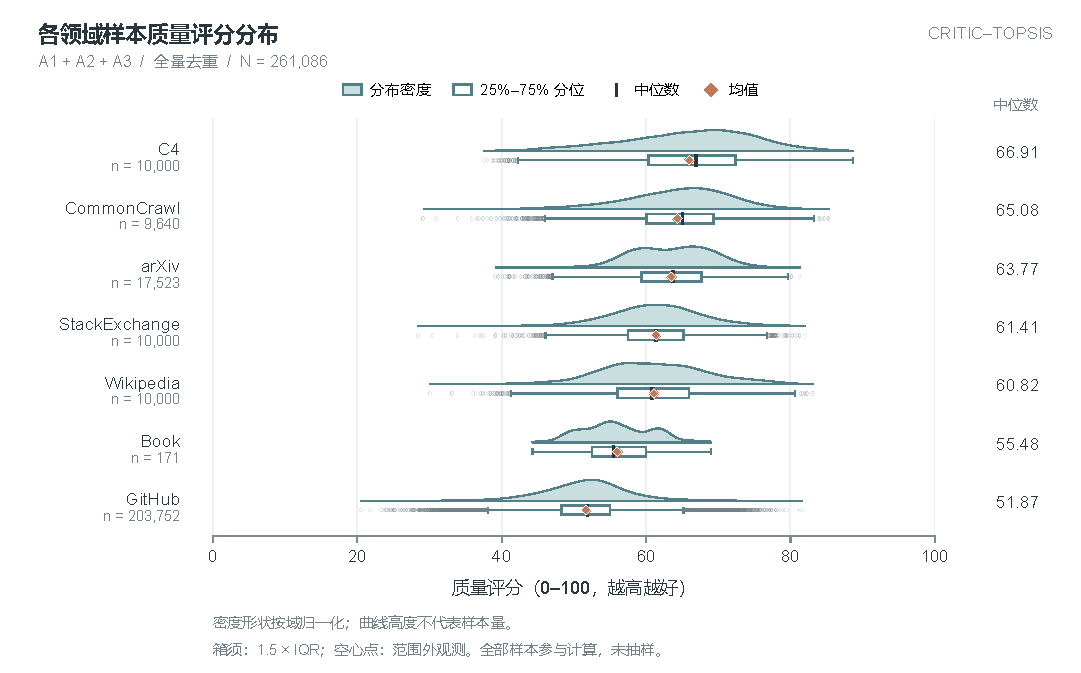
\includegraphics[width=\linewidth]{figures/q1-critic-topsis/nature-v1/figure01_domain_distribution_nature.pdf}
  \caption{全量去重语料的领域构成及抽样集对照。柱形表示各领域记录数，折线表示领域在全量语料中的占比；阴影区域标示扩展集带来的组成变化。}
  \label{fig:q1-nature-01}
\end{figure}

\paragraph{数据对象与预处理}
设第 $i$ 条记录的原始质量指标向量为 $\boldsymbol{x}_i=(x_{i1},\ldots,x_{i16})$。16 个指标覆盖语言形式、可读性、内容质量、教育性、事实性、知识覆盖与重复性等维度，其中句末标点率、cleanliness、no-ad、readability、fluency、unique words、QuRating education、writing、FineWeb education、factual、Books、Math 和 Wikipedia 为正向指标；无字母词比例、最高频二元词组占比和最高频三元词组占比为负向指标。负向指标取值较大通常意味着文本更可能由符号、模板或高频短语主导，故按噪声与重复性的代理假设作反向处理。

记方向统一后的指标为
\begin{equation}
 \widetilde{x}_{ij}=\begin{cases}
 x_{ij}, & j\in\mathcal{P},\\
 -x_{ij}, & j\in\mathcal{N},
 \end{cases}
 \qquad \mathcal{P}\cup\mathcal{N}=\{1,\ldots,16\},\quad \mathcal{P}\cap\mathcal{N}=\varnothing,
 \label{eq:q1-direction-unification}
\end{equation}
其中 $\mathcal{P}$ 和 $\mathcal{N}$ 分别为正向、负向指标集合。随后以 $A_1$ 拟合集上方向统一值的 $1\%$ 和 $99\%$ 分位数作为稳健边界 $l_j$、$u_j$，统一为“越高越好”的归一化形式
\begin{equation}
 z_{ij}=\operatorname{clip}\left(\frac{\widetilde{x}_{ij}-l_j}{u_j-l_j},0,1\right),
 \qquad
 \operatorname{clip}(t,0,1)=\min\{1,\max\{0,t\}\}.
 \label{eq:q1-robust-normalization}
\end{equation}
$A_1$ 按记录 ID 的固定哈希规则划分为 40,919 条拟合集与 10,311 条留出集；归一化边界与下文权重仅由拟合集估计，留出集及 $A_2$、$A_3$ 均不重新拟合，从而保证各集合分数可比。归一化后检查缺失值、无穷值、越界值和重复指纹，并保留每条记录的来源集、领域标签和质量分数，供后续聚合与审计。

\begin{figure}[htbp]
  \centering
  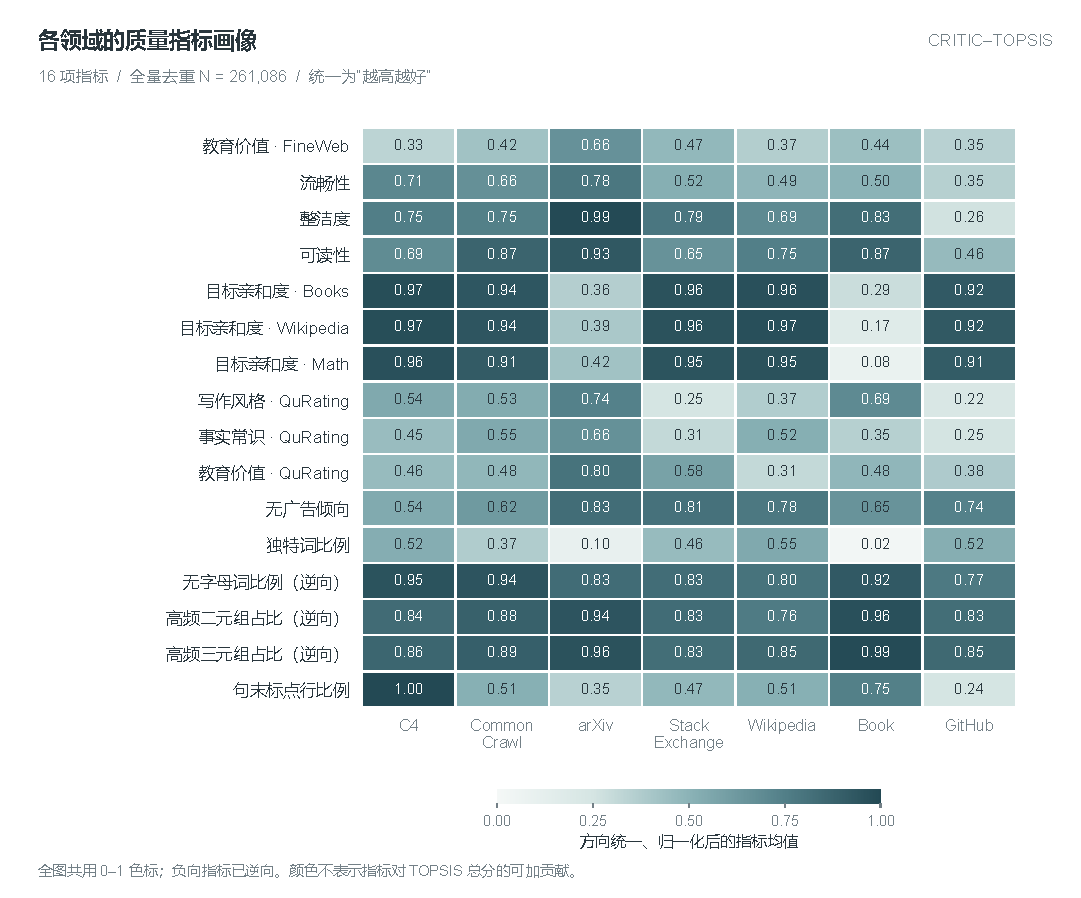
\includegraphics[width=\linewidth]{figures/q1-critic-topsis/nature-v1/figure02_indicator_heatmap_nature.pdf}
  \caption{16 个质量指标的方向统一、归一化分布及指标间相关性。颜色表示归一化后的指标水平；右侧标注负向指标在方向统一后的含义。}
  \label{fig:q1-nature-02}
\end{figure}

\paragraph{CRITIC 客观赋权}
为避免人为指定权重，采用 CRITIC 方法同时利用指标的离散程度和冲突程度。设归一化矩阵为 $Z=(z_{ij})$，第 $j$ 个指标的样本标准差为 $\sigma_j$，与第 $k$ 个指标的 Pearson 相关系数为 $r_{jk}$，则信息量为
\begin{equation}
 I_j=\sigma_j\sum_{k=1}^{16}(1-r_{jk}),\qquad
 w_j=\frac{I_j}{\sum_{m=1}^{16}I_m},\qquad
 \sum_{j=1}^{16}w_j=1.
 \label{eq:q1-critic}
\end{equation}
其中 $\sigma_j$ 反映指标对样本的区分能力，$1-r_{jk}$ 反映该指标与其他指标的信息冗余程度。权重由 $A_1$ 拟合集计算并固定用于留出集及 $A_2$、$A_3$。最终权重最高的三个指标为句末标点率（$8.91\%$）、cleanliness（$8.00\%$）和 no-ad（$7.75\%$）；三个负向词组指标合计权重为 $16.58\%$。需要说明的是，句末标点率等格式性指标权重居前，反映的是 CRITIC 以离散度与冗余度赋权的机制特征，即哪怕这些指标在样本间变异大、与其他指标冗余低，也无法证明格式特征比语义特征“更重要”；这一点在敏感性分析（图~\ref{fig:q1-nature-06}）中进一步检验。

\begin{figure}[htbp]
  \centering
  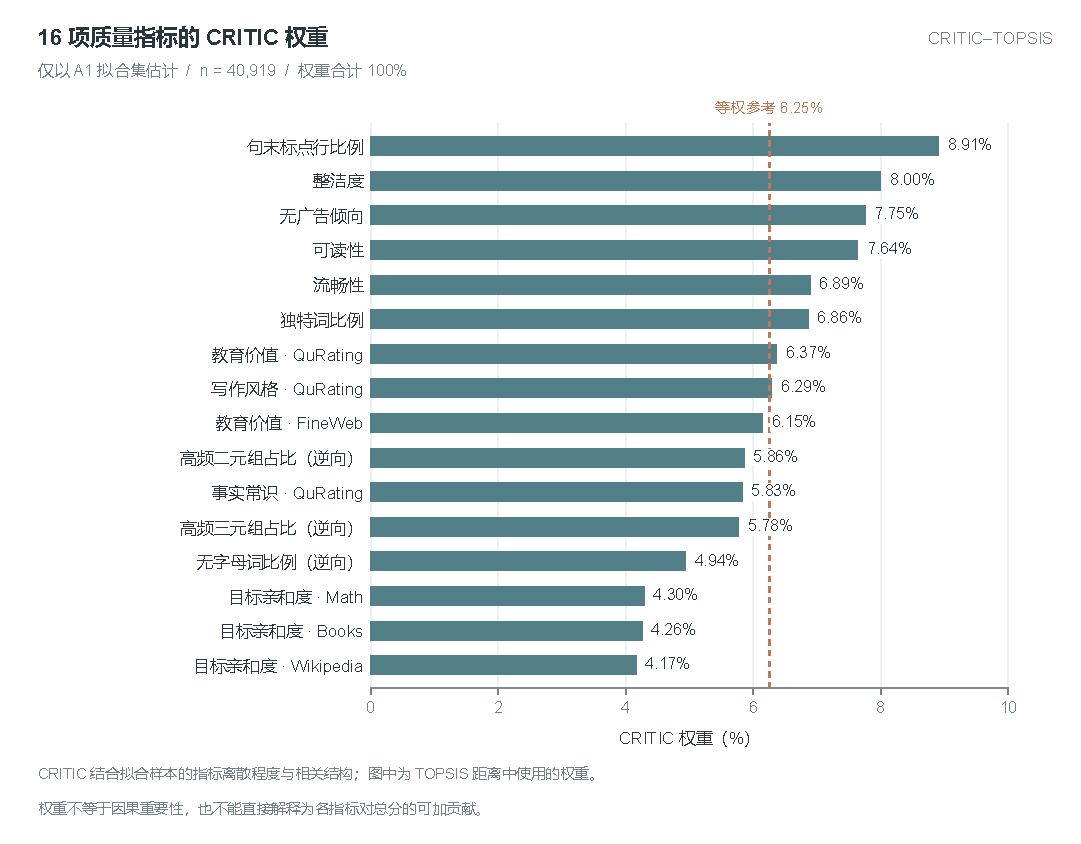
\includegraphics[width=\linewidth]{figures/q1-critic-topsis/nature-v1/figure05_critic_weights_nature.pdf}
  \caption{CRITIC 方法得到的 16 个质量指标权重。权重由 $A_1$ 拟合集估计，并固定用于全部样本。}
  \label{fig:q1-nature-05}
\end{figure}

\paragraph{加权距离 TOPSIS 评分}
以全正向理想点 $\boldsymbol{z}^{+}=\boldsymbol{1}$ 和全负向理想点 $\boldsymbol{z}^{-}=\boldsymbol{0}$ 为参照，计算第 $i$ 条记录到两类理想点的加权欧氏距离：
\begin{equation}
 D_i^{+}=\sqrt{\sum_{j=1}^{16}w_j(1-z_{ij})^2},\qquad
 D_i^{-}=\sqrt{\sum_{j=1}^{16}w_jz_{ij}^2}.
 \label{eq:q1-topsis-distance}
\end{equation}
定义样本级质量分数
\begin{equation}
 Q_i=100\times\frac{D_i^{-}}{D_i^{+}+D_i^{-}},\qquad 0\le Q_i\le100.
 \label{eq:q1-topsis-score}
\end{equation}
$Q_i$ 越大表示该记录越接近理想高质量点；在固定非负权重下，任一方向已统一的指标取值提高都不会降低 $Q_i$。因此本模型对 16 个指标采取完全可补偿的聚合立场——单指标的低分可以被其他指标的高分弥补。这一立场是明确的设计选择：它为全部样本提供单一可比标尺，但其盲区恰好是“优缺点相抵”型文本，后者由本问第二小问的冲突消解机制单独处理，两者构成递进关系。

\begin{figure}[htbp]
  \centering
  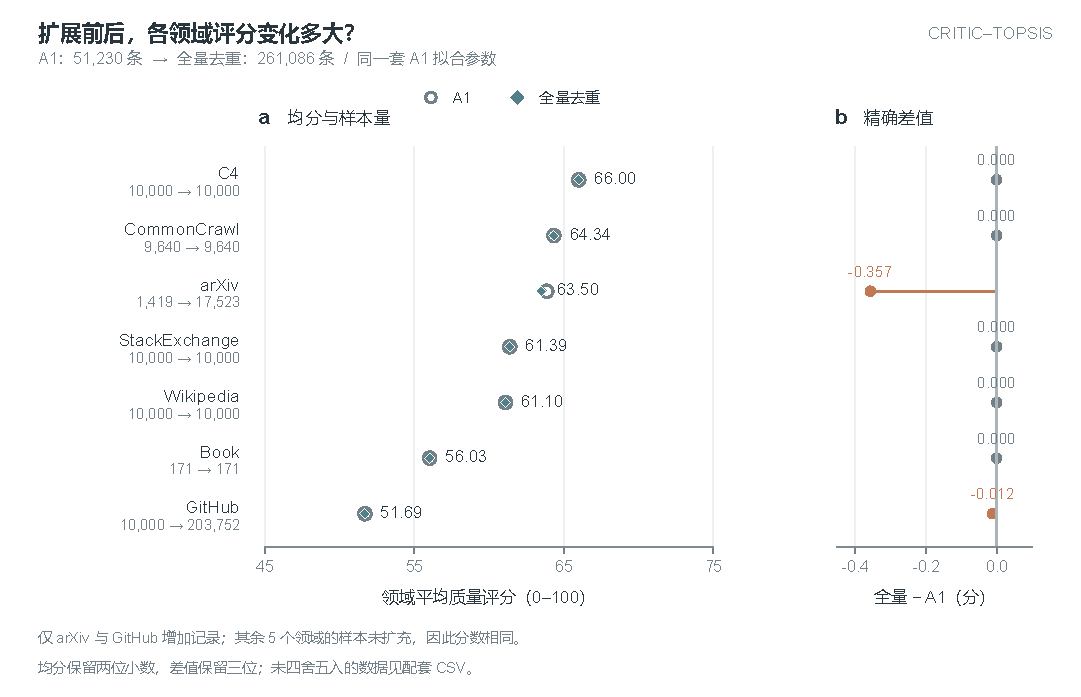
\includegraphics[width=\linewidth]{figures/q1-critic-topsis/nature-v1/figure03_A1_full_comparison_nature.pdf}
  \caption{$A_1$ 抽样集与全量去重语料的质量评分分布及分位点对照。箱线图表示中位数和四分位距，散点表示领域均值。}
  \label{fig:q1-nature-03}
\end{figure}

\paragraph{从样本级到领域级和语料级的聚合}
对领域 $g$ 的记录集合 $\mathcal{I}_g$，采用样本数加权的均值聚合：
\begin{equation}
 Q_g=\frac{1}{|\mathcal{I}_g|}\sum_{i\in\mathcal{I}_g}Q_i,
 \qquad
 Q_{\mathrm{corpus}}=\frac{1}{N}\sum_{i=1}^{N}Q_i.
 \label{eq:q1-domain-aggregation}
\end{equation}
语料级分数即全体唯一记录的算术平均。先评分后聚合的原因在于 TOPSIS 对输入非线性：将领域均值指标重新送入 TOPSIS 后，不等于样本分数的均值。均值聚合保留每条记录的等贡献原则，并将域级差异与域规模分离；中位数与四分位距作为补充统计量在附录报告。

\begin{figure}[htbp]
  \centering
  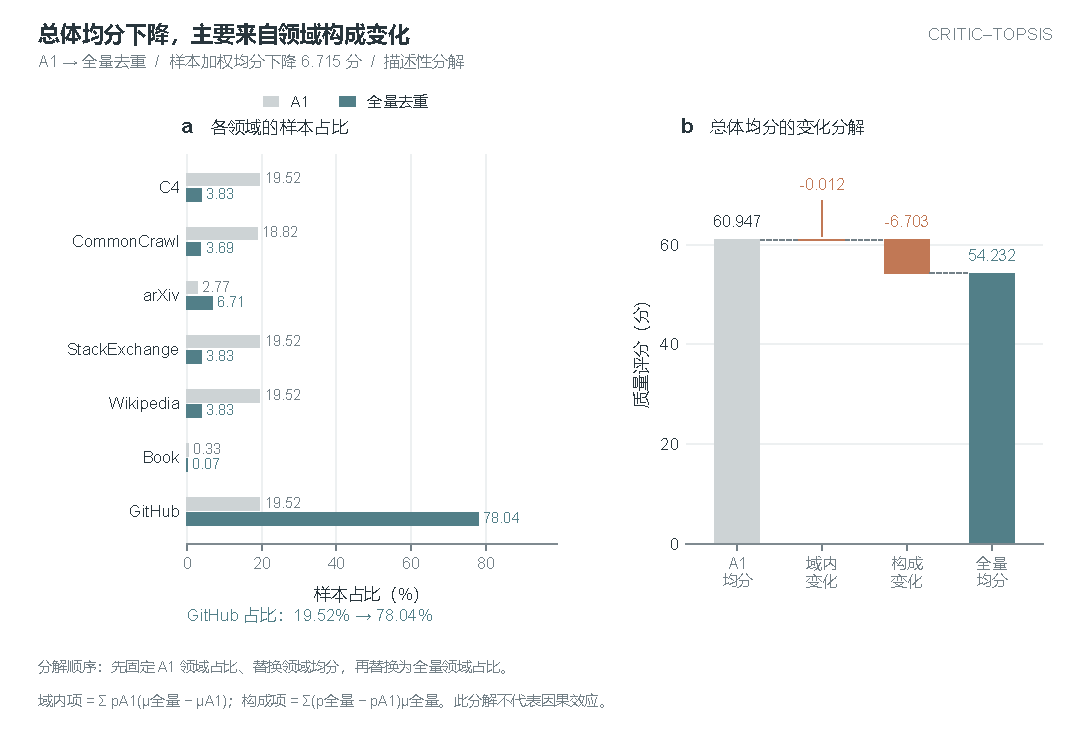
\includegraphics[width=\linewidth]{figures/q1-critic-topsis/nature-v1/figure04_composition_decomposition_nature.pdf}
  \caption{$A_1$ 到全量语料的质量变化分解。总变化分为域内质量变化与领域组成变化两部分。}
  \label{fig:q1-nature-04}
\end{figure}

\paragraph{全量结果与抽样集对照}
$A_1$ 语料级平均分为 $60.95$，全量去重语料平均分为 $54.23$，整体下降 $6.71$ 分。按领域对照：arxiv 从 $63.86$ 变为 $63.51$（下降 $0.36$ 分），github 从 $51.70$ 变为 $51.69$（下降 $0.01$ 分）；book、c4、commoncrawl、stackexchange 和 wikipedia 五个域没有新增记录，领域均值保持不变，不构成独立扩展验证。总体下降主要来自领域组成变化而非域内质量恶化：github 在 $A_1$ 中占 $19.52\%$，在全量语料中占 $78.04\%$，其较低的领域均值显著拉低了语料级分数。按“先替换领域均分、后替换领域占比”的顺序做描述性分解，域内项为 $-0.01$ 分，构成项为 $-6.70$ 分。

\begin{table}[htbp]
  \centering
  \caption{$A_1$ 与全量去重语料的领域级质量分数对照（仅 arxiv、github 两域有新增记录）}
  \label{tab:q1-domain-score}

  \renewcommand{\arraystretch}{1.15}
  \begin{tabular}{lrrrr}
    \toprule
    领域 & $A_1$ 均值 & 全量均值 & 变化 & 全量占比 \\
    \midrule
    arxiv & 63.86 & 63.51 & -0.36 & 6.71\% \\
    github & 51.70 & 51.69 & -0.01 & 78.04\% \\
    book & 56.03 & 56.03 & 0.00 & 3.55\% \\
    c4 & 66.00 & 66.00 & 0.00 & 1.02\% \\
    commoncrawl & 64.34 & 64.34 & 0.00 & 0.92\% \\
    stackexchange & 61.39 & 61.39 & 0.00 & 5.34\% \\
    wikipedia & 61.10 & 61.10 & 0.00 & 4.42\% \\
    \midrule
    语料级均值 & 60.95 & 54.23 & -6.71 & 100.00\% \\
    \bottomrule
  \end{tabular}
\end{table}

\paragraph{稳健性与适用边界}
将 CRITIC--TOPSIS 主方案与等权加权和、删除 DSIR 指标、删除三个负向词组指标三种替代方案比较。主方案与等权结果的 Spearman 秩相关系数为 $0.988$，与删 DSIR 方案为 $0.986$，与删负向指标方案为 $0.967$；在删负向指标方案中平均名次变化 $4.79$ 个百分点，约 $2.78\%$ 的样本名次变化超过 $20$ 个百分点。这表明总分的头部排序对各方案不敏感，但重复性类指标对尾部样本排序有实质影响。该敏感性检验针对的是本小问评分对建模选择的稳定性，它利用的是指标间相关性结构，与本问第二小问所处理的“同一文本上指标评价不一致”是不同概念。

\begin{figure}[htbp]
  \centering
  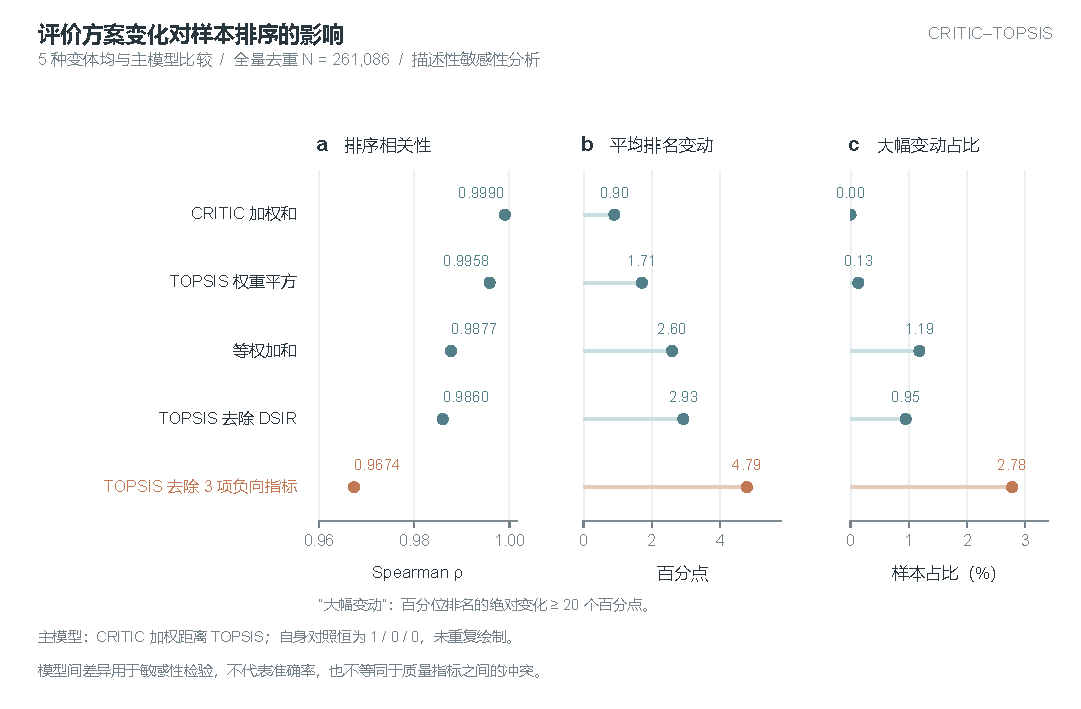
\includegraphics[width=\linewidth]{figures/q1-critic-topsis/nature-v1/figure06_model_sensitivity_nature.pdf}
  \caption{不同权重和指标删减方案下的模型敏感性。左侧展示样本分数的秩相关，右侧展示名次变化及受影响样本比例。}
  \label{fig:q1-nature-06}
\end{figure}

\paragraph{小结}
本小问形成了可复算的全量质量评价链条：以 $A_1$ 稳健边界与 CRITIC 权重建立统一标尺，以加权距离 TOPSIS 输出样本级质量分数，再按记录均值聚合为领域级与语料级分数。结果显示 $A_1$ 与全量语料在已验证域（arxiv、github）的域内质量差异不超过 $0.36$ 分，语料级均分下降的约 $99.8\%$（构成项 $-6.70$ 分，域内项 $-0.01$ 分）由领域构成变化解释。该基线一方面为第二小问的冲突消解提供输入，另一方面输出领域级质量评分 $Q_g$，经 A16 域映射引入后续配比建模与广义标度律，构成四问递进链条的第一环。
